% !TeX program = xelatex
\documentclass[11pt,a4paper]{article}
\usepackage[left=15mm,right=15mm,top=13mm,bottom=12mm]{geometry}
\usepackage{amsmath}
\usepackage{fontspec}
\usepackage{unicode-math}
\usepackage{tikz}

\setmainfont{Latin Modern Roman}
\setmathfont{Latin Modern Math}
\newfontfamily\cjkfont{Noto Serif CJK SC}
\newcommand{\zh}[1]{{\cjkfont #1}}
\newcommand{\marked}{\zh{※}\,}
\setlength{\parindent}{0pt}
\setlength{\jot}{2pt}
\pagestyle{empty}

\newcommand{\instruction}[1]{\par\noindent{\bfseries\zh{#1}}\par\vspace{2.5mm}}
\newcommand{\cell}[2]{\begin{minipage}[t]{#1}\strut #2\end{minipage}}
\newcommand{\verticalrow}[3]{%
  \noindent\cell{.30\textwidth}{#1}%
  \cell{.35\textwidth}{#2}%
  \cell{.35\textwidth}{#3}\par
}
\newcommand{\result}[1]{\ensuremath{#1}\par\vspace{1mm}}
\newcommand{\verification}{\zh{验算}\par}
\newcommand{\remainder}{\mathinner{\ldotp\ldotp\ldotp\ldotp\ldotp\ldotp}}

% 运算符和数字按位书写，\phantom{0} 为十位或百位部分积留空。
\newenvironment{verticalcalculation}[1][c]{%
  \begingroup\setlength{\arraycolsep}{2pt}\renewcommand{\arraystretch}{1.12}%
  \(\begin{array}[#1]{@{}r r@{}}%
}{\end{array}\)\endgroup}

% 除法竖式中每个横坐标单位表示一个数位。
\newlength{\divisiondigit}
\AtBeginDocument{\settowidth{\divisiondigit}{$0$}}
\tikzset{division/.style={x=\divisiondigit,y=4.35mm,line width=.45pt,
  every node/.style={anchor=east,inner sep=0pt,outer sep=0pt}}}
\newcommand{\divisionbracket}[1]{%
  \draw (-.12,.43) -- (#1,.43);
  \draw (-.12,.43) .. controls (.08,.14) and (.02,-.23) .. (-.25,-.47);
}

% 第一行保留题目，后续各行的等号对齐。
\newenvironment{steps}{\(\begin{aligned}[t]}{\end{aligned}\)}

\begin{document}
\noindent\makebox[\textwidth]{{\Large\bfseries\zh{四年级计算（答案版）}}}\par
\vspace{4mm}

\instruction{竖式计算，带※验算}
\verticalrow{%
  \result{584\times17=9928}
  \begin{verticalcalculation}
    & 584\\
    \times & 17\\ \hline
    & 4088\\
    & 584\phantom{0}\\ \hline
    & 9928
  \end{verticalcalculation}
}{%
  \marked\result{496\div32=15\remainder16}
  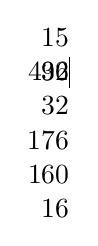
\begin{tikzpicture}[division]
    \node at (-.43,0) {$32$};
    \node at (3,1) {$15$};
    \node at (3,0) {$496$};
    \node at (2,-1) {$32$};
    \node at (3,-2) {$176$};
    \node at (3,-3) {$160$};
    \node at (3,-4) {$16$};
    \divisionbracket{3.11}
    \draw (.03,-1.52) -- (2.08,-1.52);
    \draw (.03,-3.52) -- (3.08,-3.52);
  \end{tikzpicture}\par\vspace{1mm}
  \zh{验算}\quad $16<32$\par
  \begin{verticalcalculation}[t]
    & 32\\
    \times & 15\\ \hline
    & 160\\
    & 32\phantom{0}\\ \hline
    & 480
  \end{verticalcalculation}\qquad
  \begin{verticalcalculation}[t]
    & 480\\
    + & 16\\ \hline
    & 496
  \end{verticalcalculation}
}{%
  \marked\result{333\times27=8991}
  \begin{minipage}[t]{.45\linewidth}
    \strut\par
    \begin{verticalcalculation}
      & 333\\
      \times & 27\\ \hline
      & 2331\\
      & 666\phantom{0}\\ \hline
      & 8991
    \end{verticalcalculation}
  \end{minipage}%
  \begin{minipage}[t]{.55\linewidth}
    \strut\verification
    \begin{verticalcalculation}
      & 27\\
      \times & 333\\ \hline
      & 81\\
      & 81\phantom{0}\\
      & 81\phantom{00}\\ \hline
      & 8991
    \end{verticalcalculation}
  \end{minipage}
}
\vspace{3mm}
\verticalrow{%
  \result{406\times19=7714}
  \begin{verticalcalculation}
    & 406\\
    \times & 19\\ \hline
    & 3654\\
    & 406\phantom{0}\\ \hline
    & 7714
  \end{verticalcalculation}
}{%
  \marked\result{1047\div35=29\remainder32}
  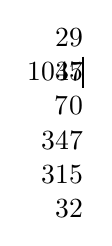
\begin{tikzpicture}[division]
    \node at (-.43,0) {$35$};
    \node at (4,1) {$29$};
    \node at (4,0) {$1047$};
    \node at (3,-1) {$70$};
    \node at (4,-2) {$347$};
    \node at (4,-3) {$315$};
    \node at (4,-4) {$32$};
    \divisionbracket{4.11}
    \draw (.03,-1.52) -- (3.08,-1.52);
    \draw (1.03,-3.52) -- (4.08,-3.52);
  \end{tikzpicture}\par\vspace{1mm}
  \zh{验算}\quad $32<35$\par
  \begin{verticalcalculation}[t]
    & 35\\
    \times & 29\\ \hline
    & 315\\
    & 70\phantom{0}\\ \hline
    & 1015
  \end{verticalcalculation}\qquad
  \begin{verticalcalculation}[t]
    & 1015\\
    + & 32\\ \hline
    & 1047
  \end{verticalcalculation}
}{%
  \result{817\times36=29412}
  \begin{verticalcalculation}
    & 817\\
    \times & 36\\ \hline
    & 4902\\
    & 2451\phantom{0}\\ \hline
    & 29412
  \end{verticalcalculation}
}
\vspace{5mm}

\instruction{脱式计算，能简算的要简算}
\noindent\cell{.27\textwidth}{%
  \begin{steps}
    &\phantom{{}={}}99\times99+99\\
    &=99\times99+99\times1\\
    &=99\times(99+1)\\
    &=99\times100\\
    &=9900
  \end{steps}
}%
\cell{.38\textwidth}{%
  \begin{steps}
    &\phantom{{}={}}25\times(19+19+19+19)\\
    &=25\times(4\times19)\\
    &=(25\times4)\times19\\
    &=100\times19\\
    &=1900
  \end{steps}
}%
\cell{.35\textwidth}{%
  \begin{steps}
    &\phantom{{}={}}840\div7\times(36-11)\\
    &=840\div7\times25\\
    &=120\times25\\
    &=(30\times4)\times25\\
    &=30\times(4\times25)\\
    &=30\times100\\
    &=3000
  \end{steps}
}\par\vspace{3mm}

\noindent\cell{.60\textwidth}{%
  \begin{steps}
    &\phantom{{}={}}502\times[1020\div(960-940)]\\
    &=502\times[1020\div20]\\
    &=502\times51\\
    &=(500+2)\times51\\
    &=500\times51+2\times51\\
    &=25500+102\\
    &=25602
  \end{steps}
}%
\cell{.40\textwidth}{%
  \begin{steps}
    &\phantom{{}={}}816\div[(19-11)\times6]\\
    &=816\div[8\times6]\\
    &=816\div48\\
    &=17
  \end{steps}
}\par\vspace{3mm}

\noindent\cell{.67\textwidth}{%
  \begin{steps}
    &\phantom{{}={}}99+999+9999+99999\\
    &=(100-1)+(1000-1)+(10000-1)+(100000-1)\\
    &=100+1000+10000+100000-4\\
    &=111100-4\\
    &=111096
  \end{steps}
}%
\cell{.33\textwidth}{%
  \begin{steps}
    &\phantom{{}={}}738-301\\
    &=738-(300+1)\\
    &=738-300-1\\
    &=438-1\\
    &=437
  \end{steps}
}\par
\end{document}
